 \documentclass[11pt, oneside]{article} 
\usepackage{geometry}
\geometry{letterpaper} 
\usepackage{graphicx}
	
\usepackage{amssymb}
\usepackage{amsmath}
\usepackage{parskip}
\usepackage{color}
\usepackage{hyperref}

\graphicspath{{/Users/telliott_admin/Dropbox/Tex/png/}}
% \begin{center} 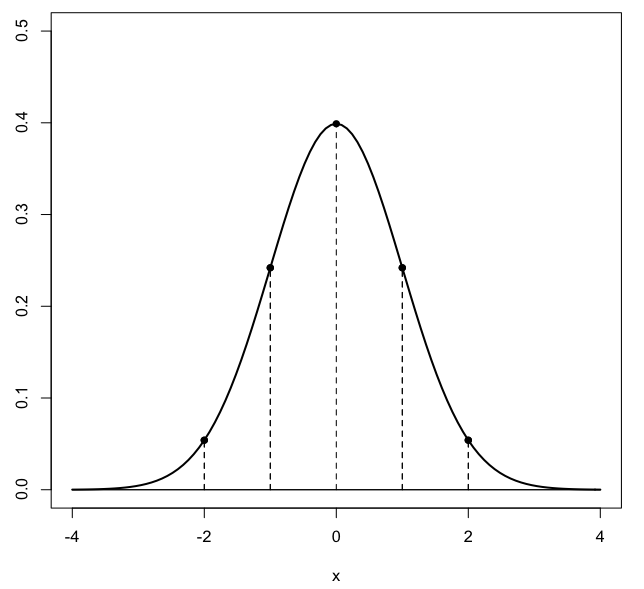
\includegraphics [scale=0.4] {gauss3.png} \end{center}

\title{Countable sets}
\date{}

\begin{document}
\maketitle
\Large

\textbf{Eternity is a very long time, especially towards the end. }

(credited to Woody Allen)

\subsection*{infinity}

The supply of natural numbers $\mathbb{N}$ is infinite, because if not, then there would be a maximum integer $m \in \mathbb{N}$.  But $m + 1$ is also $\in \mathbb{N}$, and $m+1 > m$, which is a contradiction.

Both the real numbers and the rational numbers also come in an infinite supply, for basically the same reason.  Just add $1$ to the "maximum" $m$, then find a real or a rational in the interval $(m,m+1)$.  

Even for a finite interval such as $(0,1)$, the properties described above prove that this finite interval contains an infinite number of both rational and real numbers.

But more than this, in an important sense, there are \emph{many more} real numbers than rational numbers.

\subsection*{more reals}

\url{www-history.mcs.st-and.ac.uk/~john/analysis/Lectures/L4.html}

The set $\mathbb{N}$ is \textbf{countable}.  Any set that can be put into one-to-one correspondence with $\mathbb{N}$ is also countable.

The set $\mathbb{Z}$ is countable:

\begin{center} 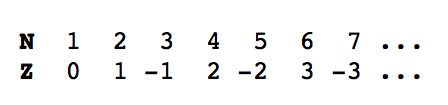
\includegraphics [scale=0.5] {Z_count.png} \end{center}

The set $\mathbb{N \times N}$ is countable:

\begin{center} 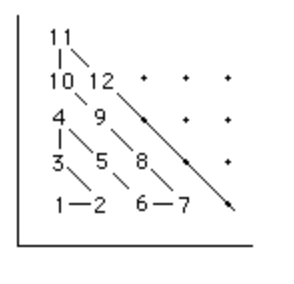
\includegraphics [scale=0.5] {countable.png} \end{center}

Count the points with integer coefficients in the positive quadrant as shown above.

The set $\mathbb{Q}$ is countable:

The idea of the proof is to show that one can set up a correspondence between $\mathbb{N}$ and $\mathbb{Q}$, assigning each number $r \in \mathbb{Q}$ in a particular order to $1,2,3, \dots$.  Here is the figure from Courant and John:
\begin{center} 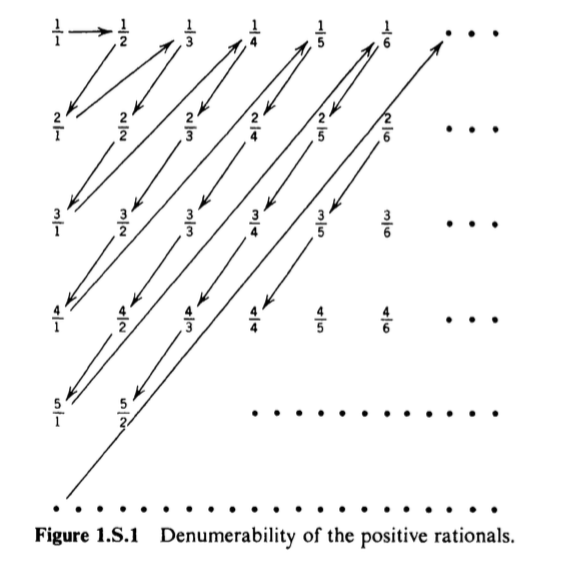
\includegraphics [scale=0.6] {denumerability.png} \end{center}

We first set up the sequence
\[ \frac{1}{1} \ \ \ \frac{1}{2}, \frac{2}{1} \ \ \  \frac{1}{3}, \frac{2}{2}, \frac{3}{1} \ \ \ \frac{1}{4}, \frac{2}{3}, \frac{3}{2}, \frac{4}{1} \ \ \ \frac{1}{5}, \frac{2}{4}, \frac{3}{3}, \frac{4}{2}, \frac{5}{1} \ \ \  \frac{1}{6}, \frac{2}{5}, \frac{3}{4}, \frac{4}{3}, \frac{5}{2}, \frac{6}{1} \dots \]
Then we remove all fractions that are duplicates by way of not being in lowest terms.
\[ \frac{1}{1} \ \ \ \frac{1}{2}, \frac{2}{1} \ \ \  \frac{1}{3}, \frac{3}{1} \ \ \ \frac{1}{4}, \frac{2}{3}, \frac{3}{2}, \frac{4}{1} \ \ \ \frac{1}{5}, \frac{5}{1} \ \ \  \frac{1}{6}, \frac{2}{5}, \frac{3}{4}, \frac{4}{3}, \frac{5}{2}, \frac{6}{1} \dots \]

Finally, each $r$ in this sequence is assigned to a natural number (in the sequence $\mathbb{N}$), establishing the denumerability property.

Cantor showed that such a correspondence is impossible for $\mathbb{R}$.  The proof of this is is not hard.  You can check out the chapters on Georg Cantor in Dunham's \emph{Journey Through Genius}.

We will show that the set of reals in the interval $(0,1)$ is not countable.

The proof is called the \emph{Cantor diagonalization argument}.

Suppose we could write down all the decimal expansions of the reals in the interval $(0,1)$ in a list:

$0. a_1 \ a_2 \ a_3 \ a_4 \ a_5 \dots$

$0. b_1 \ b_2 \ b_3 \ b_4 \ b_5 \dots$

$0. c_1 \ c_2 \ c_3 \ c_4 \ c_5 \dots$

$0. d_1 \ d_2 \ d_3 \ d_4 \ d_5 \dots$

$\dots$

Then this list would be countable, but it does not contain all the reals in the interval $(0,1)$

Define a decimal $x = x_1 \ x_2 \ x_3 \ x_4 \ \dots$, with $x_1 \ne a_1$ and also $x_1 \ne 9$ (so $x$ doesn't end in recurring $9$'s), then $x_2 \ne b_2,9$, $x_3 \ne c_3,9$, etc.

Then the decimal expansion of $x$ does not end in recurring $9$'s and it differs from the nth element of the list in the nth decimal place. Hence it represents an element of the interval (0, 1) which is not in our counting and so we do not have a counting of the reals in (0, 1).

Thus, the rational numbers are said to be "countably infinite", while the real numbers are not countable.  

A real number is called algebraic if it is a root of a polynomial with rational (or integer) coefficients. Other real numbers are called transcendental.  There is also a proof that the transcendental numbers are much more numerous than the non-transcendental ones.

\end{document}